%% ------------------------------------------------------------------
%% Cover Letter — EPFL, Full Stack Software Engineer (School of Engineering)
%% Reference: 2357
%%
%% Based on applications/_shared/latex/cover-letter-template.tex
%% Compile: pdflatex cover-letter.tex (twice for hyperref cross-refs)
%% ------------------------------------------------------------------

\documentclass[11pt,a4paper]{article}

%% ------- Font and encoding (mirrors the CV) -------
\usepackage[utf8]{inputenc}
\usepackage[T1]{fontenc}
\usepackage[default]{lato}

%% ------- Layout -------
\usepackage[a4paper, top=1.5cm, bottom=1.75cm, left=2cm, right=2cm]{geometry}
\usepackage{parskip}
\setlength{\parindent}{0pt}
\setlength{\parskip}{0.75em}
\renewcommand{\baselinestretch}{1.15}

%% ------- Ragged right -------
\usepackage[document]{ragged2e}

%% ------- Hyperlinks -------
\usepackage{hyperref}

%% ------- Shared visual identity -------
%% ------------------------------------------------------------------
%% identity.tex — Shared visual identity for CV and cover letters
%%
%% \input this file from any LaTeX document that should share the
%% Gonçalves visual identity (colors, icons, tipography helpers,
%% graphics search paths).
%%
%% Idempotent by design: safe to \input from documents that already
%% loaded xcolor / fontawesome / graphicx (via altacv or otherwise).
%% Uses \providecommand for macros so re-\input never errors.
%%
%% Callers currently include:
%%   - applications/_shared/latex/cover-letter-template.tex
%%   - applications/YYYY-MM-<slug>/cover-letter.tex (copied from template)
%%   - Optionally the CV itself, if the shared identity refactor is applied.
%% ------------------------------------------------------------------

%% ------- Required packages (loaded only if not already loaded) -------
\makeatletter
\@ifpackageloaded{xcolor}{}{\usepackage{xcolor}}
\@ifpackageloaded{fontawesome}{}{\usepackage{fontawesome}}
\@ifpackageloaded{graphicx}{}{\usepackage{graphicx}}
\@ifpackageloaded{tikz}{}{\usepackage{tikz}}
\makeatother

%% ------- Color palette (same values used by curriculum-en.tex) -------
\definecolor{StPatricksBlue}{HTML}{1F3D77}
\definecolor{SlateGrey}{HTML}{2E2E2E}
\definecolor{LightGrey}{HTML}{333333}

%% ------- Graphics search paths -------
%% Lets 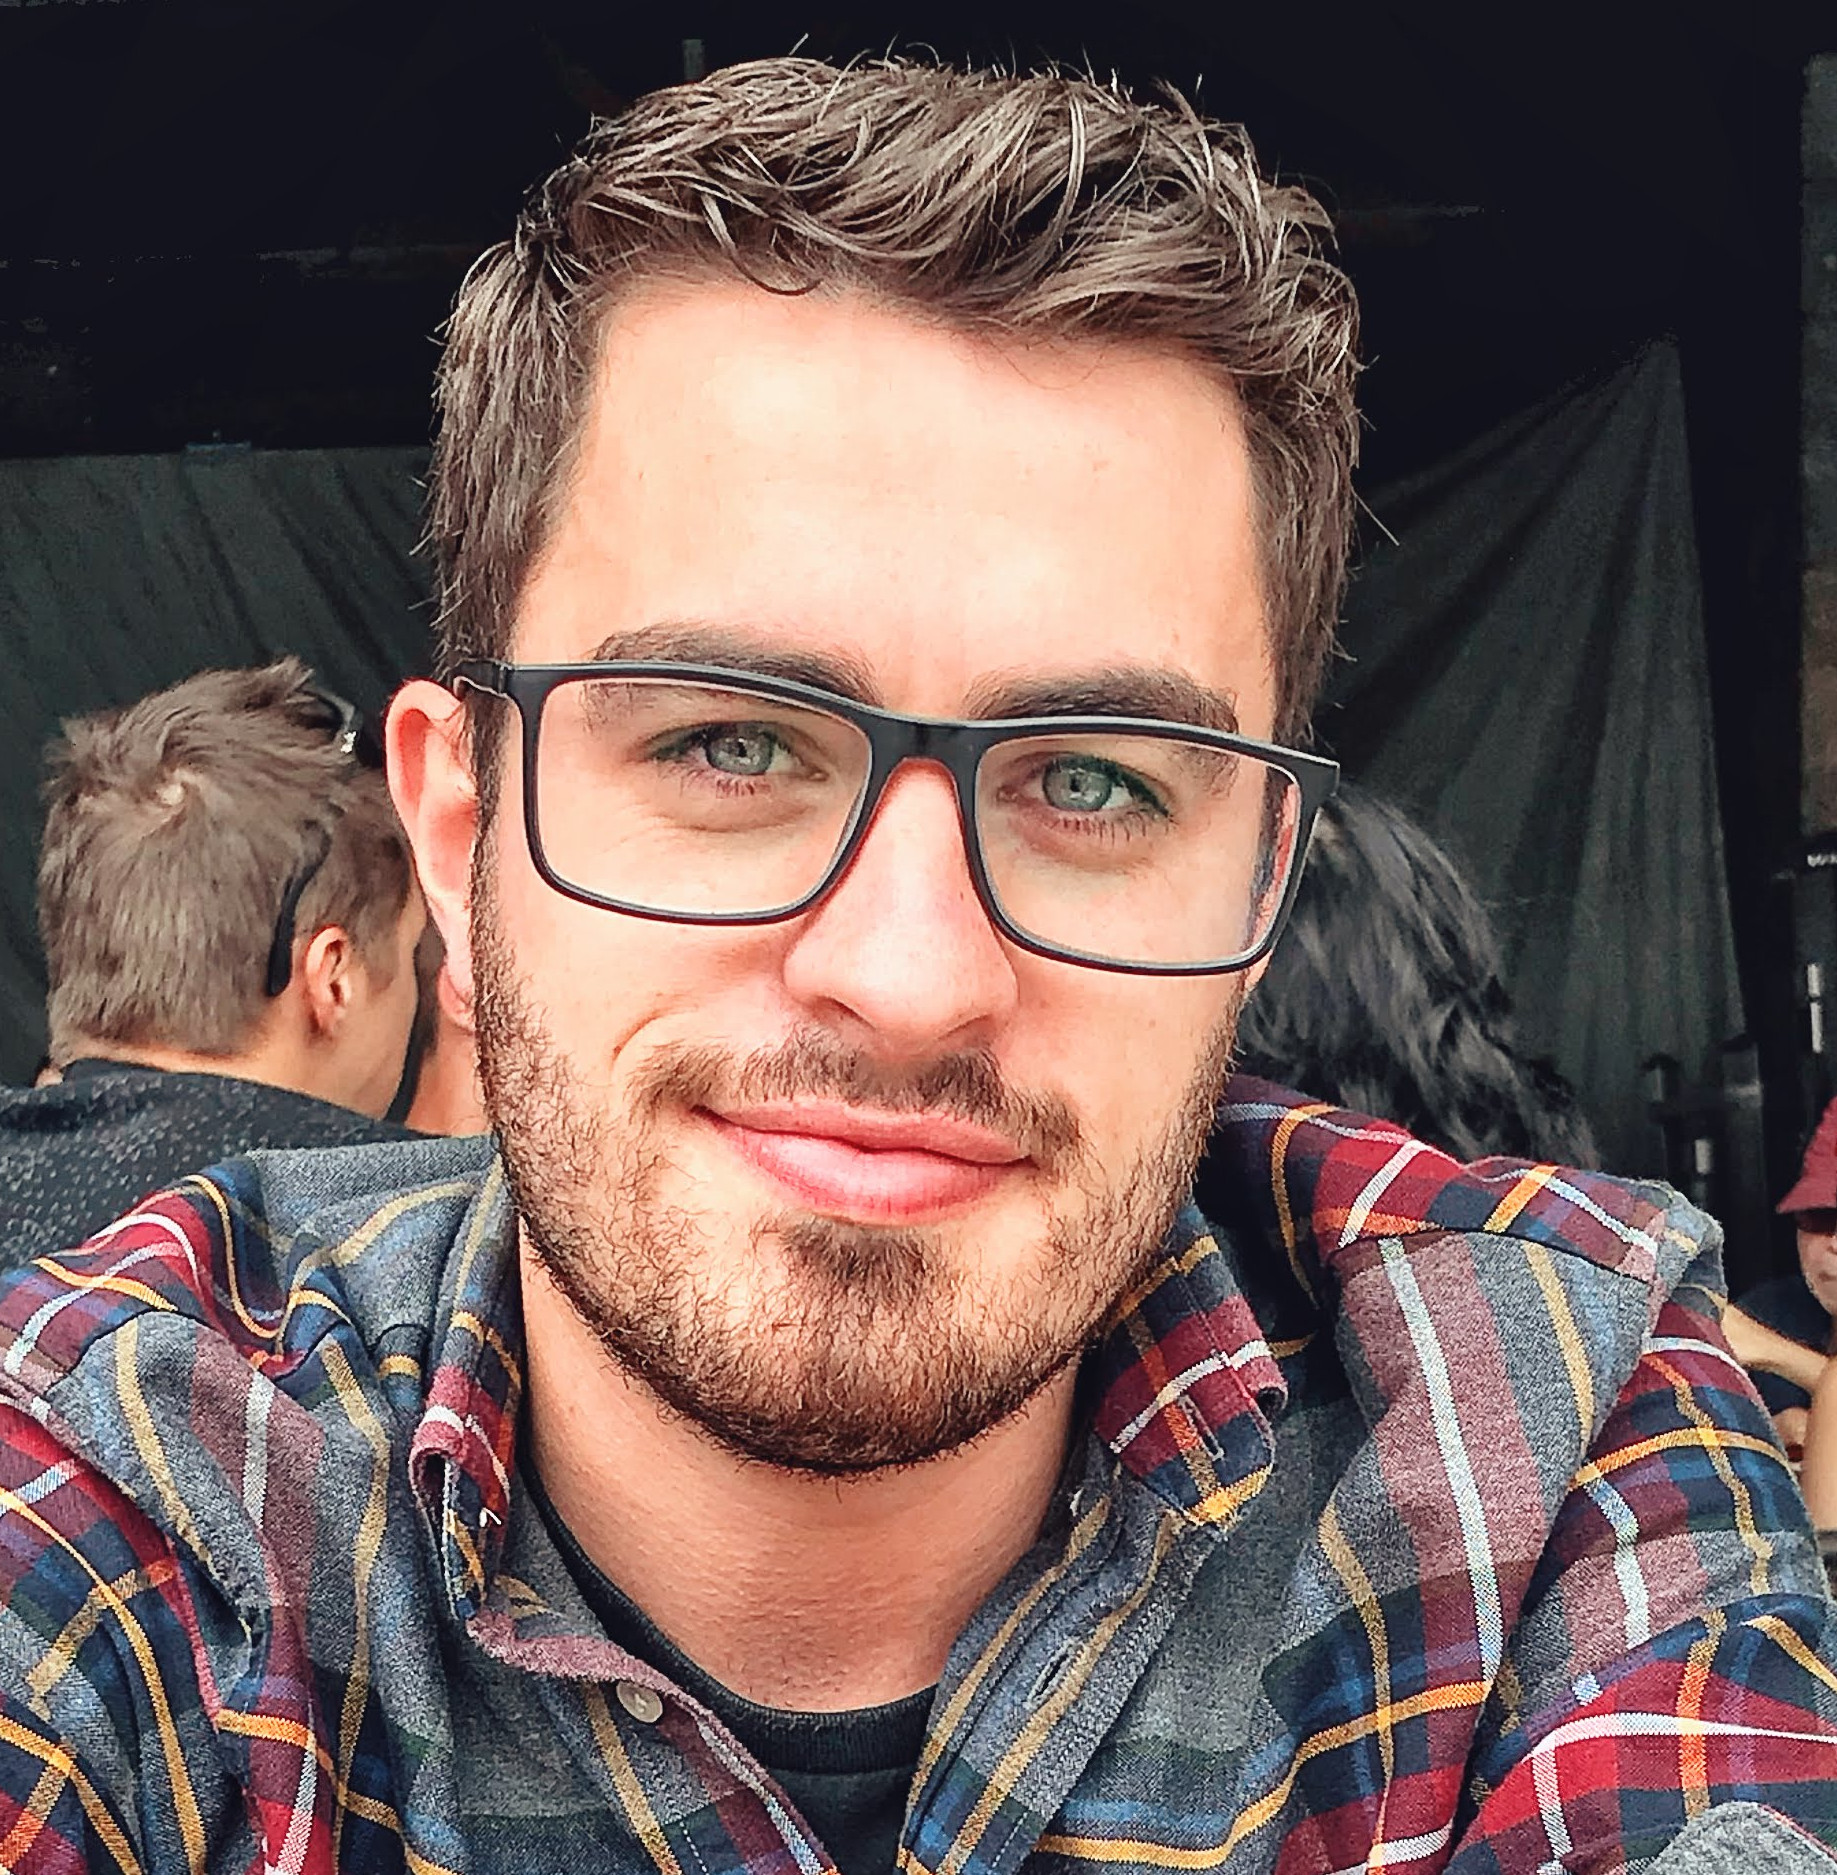
\includegraphics{profile} resolve to english/profile.jpg from any
%% depth the caller might be at. LaTeX tries these in order and uses the
%% first match.
\graphicspath{%
    {./}%                          same folder as the caller
    {./english/}%                  from project root
    {../english/}%                 from applications/ (unlikely, but cheap)
    {../../english/}%              from applications/YYYY-MM-<slug>/
    {../../../english/}%           from applications/_shared/latex/
}

%% ------- Style helpers for cover letters -------
%% Not used by the CV (altacv defines its own header macros), but harmless
%% to have loaded. \providecommand only defines if not already defined.

\providecommand{\senderName}[1]{%
    {\fontsize{22pt}{28pt}\selectfont\bfseries\color{StPatricksBlue}#1}%
}

\providecommand{\senderTagline}[1]{%
    {\fontsize{11pt}{14pt}\selectfont\itshape\color{SlateGrey}#1}%
}

\providecommand{\contactBullet}{%
    \hspace{0.5em}\textcolor{StPatricksBlue}{$\bullet$}\hspace{0.5em}%
}

\providecommand{\dividerLine}{%
    {\color{StPatricksBlue}\rule{\linewidth}{0.6pt}}%
}

\providecommand{\salutation}[1]{%
    {\bfseries\color{SlateGrey}#1}%
}

\providecommand{\closing}[1]{%
    {\bfseries\color{SlateGrey}#1}%
}

%% ------- Date and subject-line helpers for cover letters -------

%% \letterDate{City}
%% Renders "City, DD Month YYYY" right-aligned, in italic SlateGrey. Uses
%% \today under the hood so the date is always current at compile time.
%% Example: \letterDate{Lausanne}  ->  "Lausanne, 27 July 2026"
\providecommand{\letterMonth}{%
    \ifcase\month\or January\or February\or March\or April\or May\or June%
    \or July\or August\or September\or October\or November\or December\fi%
}
\providecommand{\letterDate}[1]{%
    \hfill{\itshape\color{SlateGrey}#1,~\the\day~\letterMonth~\the\year}%
}

%% \subjectLine{content}
%% Renders a bold SlateGrey subject line. Common convention in formal
%% European/Swiss/French letters (e.g. "Subject: ..." or "Object: ...").
%% The caller decides whether to include a prefix.
%% Example: \subjectLine{Subject: Application for Full Stack Engineer -- Ref. 2357}
\providecommand{\subjectLine}[1]{%
    {\bfseries\color{SlateGrey}#1}%
}

%% ------- Circular photo (matches altacv's \photo behavior in the CV) -------
%% \circularPhoto{diameter}{filename}
%% Renders a circular-cropped photo, resolving the filename via \graphicspath
%% (so \circularPhoto{2.5cm}{profile} finds english/profile.jpg).
%% The tikzpicture baseline is set to the top of the circle so that when used
%% inside a minipage with [t] alignment, the picture aligns with the top of
%% the row rather than the middle of the circle (default tikz behavior).
%% Example: \circularPhoto{2.5cm}{profile}
\providecommand{\circularPhoto}[2]{%
    \begin{tikzpicture}[baseline=(currentphoto.north)]
        \node[circle,minimum size=#1,inner sep=0pt,%
            path picture={%
                \node[inner sep=0pt] at (path picture bounding box.center) {%
                    \includegraphics[width=#1]{#2}%
                };%
            }%
        ] (currentphoto) {};
    \end{tikzpicture}%
}


\hypersetup{
    colorlinks=true,
    urlcolor=StPatricksBlue,
    linkcolor=StPatricksBlue,
    pdftitle={Guilherme I. Goncalves - Cover Letter - EPFL},
    pdfauthor={Guilherme I. Goncalves}
}

\color{LightGrey}

%% ==================================================================
\begin{document}

%% ------- HEADER: name + tagline + contact info (left) + circular photo (right) -------
%% Uses explicit dimensions to guarantee side-by-side layout:
%%   text minipage = linewidth - 3cm (leaves room for photo + gap)
%%   photo minipage = 2.7cm (2.5cm photo + 0.2cm buffer)
%%   \hfill absorbs the ~0.3cm remaining slack

\noindent%
\begin{minipage}[t]{\dimexpr\linewidth-3cm\relax}%
\senderName{Guilherme Inácio Gonçalves, Ph.D.}\\[0.4em]
\senderTagline{Senior Full-Stack Software Engineer}\\[0.8em]
{\color{LightGrey}\small
\faEnvelope\ \href{mailto:ginaciog@cern.ch}{ginaciog@cern.ch}\contactBullet%
\faPhone\ +55 22 99923 1446\contactBullet%
\faMapMarker\ Nova Friburgo, Brazil\\[0.3em]
\faLinkedin\ \href{https://linkedin.com/in/inacioguilherme}{linkedin.com/in/inacioguilherme}\contactBullet%
\faGithub\ \href{https://github.com/ingoncalves}{github.com/ingoncalves}
}%
\end{minipage}%
\hfill%
\begin{minipage}[t]{2.7cm}%
\circularPhoto{2.5cm}{profile}%
\end{minipage}%
\par

\vspace{0.75em}
\dividerLine
\vspace{1.25em}

%% ------- DATE -------

\letterDate{Lausanne}

\vspace{1em}

%% ------- RECIPIENT BLOCK -------

{\color{SlateGrey}
Human Resources — Recruitment\\
School of Engineering (STI)\\
EPFL — École polytechnique fédérale de Lausanne\\
CH-1015 Lausanne, Switzerland
}

\vspace{1.25em}

%% ------- SUBJECT LINE -------

\subjectLine{Subject: Application for Full Stack Software Engineer (Reference 2357)}

\vspace{1em}

%% ------- SALUTATION -------

\salutation{Dear Hiring Team,}

%% ------- BODY -------

I am applying for the Full Stack Software Engineer position with the School of Engineering because EPFL sits at an unusually specific intersection of things I have spent my career building toward: rigorous scientific software, full-stack production engineering, open-source contribution, and modern AI-agentic development practices.

Since 2019 I have been a CERN user on the ATLAS Tile Calorimeter, working within the Athena open-source software framework and achieving full ATLAS authorship in 2024. In February 2026 I defended my PhD in Computational Modeling, with research on signal estimation for high-energy calorimeters under HL-LHC luminosity conditions. The PhD produced two open-source contributions used internationally by the high-energy physics community: the calorimetry-pulse-simulator library and Lorenzetti, a general-purpose calorimetry simulation framework I co-developed and published in Elsevier in 2023. I have also contributed upstream to Athena, Etherpad, and Scilab. This scientific background gives me a natural cultural fit with EPFL as a peer institution to CERN.

In parallel, I have spent the past decade as a full-stack engineer in industry. I am currently a Senior Full-Stack Engineer at Siteimprove, a global SaaS platform for digital accessibility and content quality, where I work daily with Node.js, TypeScript, React, Java (Spring Boot), and cloud-native architecture on AWS. I also recently co-founded Orkast, a multi-tenant SaaS platform where, as sole engineer, I own the full stack end-to-end: PostgreSQL with a full ORM layer, a NestJS back-end, a React front-end, Docker-based deployments on ECS Fargate, and the entire infrastructure defined in Terraform. I build daily with Claude Code as a first-class part of my engineering workflow.

Regarding the position at the School of Engineering specifically, the technology stack overlaps completely with my day-to-day work: React.js, Node.js, PostgreSQL, Docker, Kubernetes, and CI/CD are tools I use to deploy applications to production on a weekly basis. I have extensive experience with Python, gained during my scientific work at CERN; although I have not yet deployed a FastAPI application to production, its modern, asynchronous architecture and Pydantic-centered typing discipline align with how I already work with other stacks, such as Node.js/TypeScript, Spring Boot/Java, and .NET/C\#, giving me comprehensive experience in web software development. I am also actively engaged in security-conscious development: I am part of Siteimprove's FedRAMP certification effort, where I triage security findings across more than 200 repositories and ship remediation code into production. The Zero Trust and Least Privilege principles mentioned in the posting are principles I apply in practice every day.

Beyond stack, the emphasis on Agentic Workflows and AI-driven development in the role description matches exactly how I have been working in my daily practice at Orkast, where I integrate Claude Code into my engineering loop and Anthropic Claude API into product features. I am eager to bring this practice into an institutional research context.

What draws me to EPFL beyond the technical fit is the mission and the environment. Empowering education and research through impactful software is a mission that compounds; it aligns directly with the values I articulated to myself when I joined the CERN community six years ago. I hold a DELF B2 diploma in French and lived in Geneva during my initial CERN period in 2019 and 2020, so the language and cultural transition to Lausanne is one I am prepared for. My family (spouse and one-year-old daughter) is fully aligned with the relocation.

I would welcome the opportunity to discuss how my background could contribute to the School of Engineering team. Thank you for your consideration.

\vspace{1em}

\closing{Sincerely,}

\vspace{2em}

\textbf{Guilherme Gonçalves}

\end{document}
